\documentclass[1p]{elsarticle_modified}
%\bibliographystyle{elsarticle-num}

%\usepackage[colorlinks]{hyperref}
%\usepackage{abbrmath_seonhwa} %\Abb, \Ascr, \Acal ,\Abf, \Afrak
\usepackage{amsfonts}
\usepackage{amssymb}
\usepackage{amsmath}
\usepackage{amsthm}
\usepackage{scalefnt}
\usepackage{amsbsy}
\usepackage{kotex}
\usepackage{caption}
\usepackage{subfig}
\usepackage{color}
\usepackage{graphicx}
\usepackage{xcolor} %% white, black, red, green, blue, cyan, magenta, yellow
\usepackage{float}
\usepackage{setspace}
\usepackage{hyperref}

\usepackage{tikz}
\usetikzlibrary{arrows}

\usepackage{multirow}
\usepackage{array} % fixed length table
\usepackage{hhline}

%%%%%%%%%%%%%%%%%%%%%
\makeatletter
\renewcommand*\env@matrix[1][\arraystretch]{%
	\edef\arraystretch{#1}%
	\hskip -\arraycolsep
	\let\@ifnextchar\new@ifnextchar
	\array{*\c@MaxMatrixCols c}}
\makeatother %https://tex.stackexchange.com/questions/14071/how-can-i-increase-the-line-spacing-in-a-matrix
%%%%%%%%%%%%%%%

\usepackage[normalem]{ulem}

\newcommand{\msout}[1]{\ifmmode\text{\sout{\ensuremath{#1}}}\else\sout{#1}\fi}
%SOURCE: \msout is \stkout macro in https://tex.stackexchange.com/questions/20609/strikeout-in-math-mode

\newcommand{\cancel}[1]{
	\ifmmode
	{\color{red}\msout{#1}}
	\else
	{\color{red}\sout{#1}}
	\fi
}

\newcommand{\add}[1]{
	{\color{blue}\uwave{#1}}
}

\newcommand{\replace}[2]{
	\ifmmode
	{\color{red}\msout{#1}}{\color{blue}\uwave{#2}}
	\else
	{\color{red}\sout{#1}}{\color{blue}\uwave{#2}}
	\fi
}

\newcommand{\Sol}{\mathcal{S}} %segment
\newcommand{\D}{D} %diagram
\newcommand{\A}{\mathcal{A}} %arc


%%%%%%%%%%%%%%%%%%%%%%%%%%%%%5 test

\def\sl{\operatorname{\textup{SL}}(2,\Cbb)}
\def\psl{\operatorname{\textup{PSL}}(2,\Cbb)}
\def\quan{\mkern 1mu \triangleright \mkern 1mu}

\theoremstyle{definition}
\newtheorem{thm}{Theorem}[section]
\newtheorem{prop}[thm]{Proposition}
\newtheorem{lem}[thm]{Lemma}
\newtheorem{ques}[thm]{Question}
\newtheorem{cor}[thm]{Corollary}
\newtheorem{defn}[thm]{Definition}
\newtheorem{exam}[thm]{Example}
\newtheorem{rmk}[thm]{Remark}
\newtheorem{alg}[thm]{Algorithm}

\newcommand{\I}{\sqrt{-1}}
\begin{document}

%\begin{frontmatter}
%
%\title{Boundary parabolic representations of knots up to 8 crossings}
%
%%% Group authors per affiliation:
%\author{Yunhi Cho} 
%\address{Department of Mathematics, University of Seoul, Seoul, Korea}
%\ead{yhcho@uos.ac.kr}
%
%
%\author{Seonhwa Kim} %\fnref{s_kim}}
%\address{Center for Geometry and Physics, Institute for Basic Science, Pohang, 37673, Korea}
%\ead{ryeona17@ibs.re.kr}
%
%\author{Hyuk Kim}
%\address{Department of Mathematical Sciences, Seoul National University, Seoul 08826, Korea}
%\ead{hyukkim@snu.ac.kr}
%
%\author{Seokbeom Yoon}
%\address{Department of Mathematical Sciences, Seoul National University, Seoul, 08826,  Korea}
%\ead{sbyoon15@snu.ac.kr}
%
%\begin{abstract}
%We find all boundary parabolic representation of knots up to 8 crossings.
%
%\end{abstract}
%\begin{keyword}
%    \MSC[2010] 57M25 
%\end{keyword}
%
%\end{frontmatter}

%\linenumbers
%\tableofcontents
%
\newcommand\colored[1]{\textcolor{white}{\rule[-0.35ex]{0.8em}{1.4ex}}\kern-0.8em\color{red} #1}%
%\newcommand\colored[1]{\textcolor{white}{ #1}\kern-2.17ex	\textcolor{white}{ #1}\kern-1.81ex	\textcolor{white}{ #1}\kern-2.15ex\color{red}#1	}

{\Large $\underline{12a_{0732}~(K12a_{0732})}$}

\setlength{\tabcolsep}{10pt}
\renewcommand{\arraystretch}{1.6}
\vspace{1cm}\begin{tabular}{m{100pt}>{\centering\arraybackslash}m{274pt}}
\multirow{5}{120pt}{
	\centering
	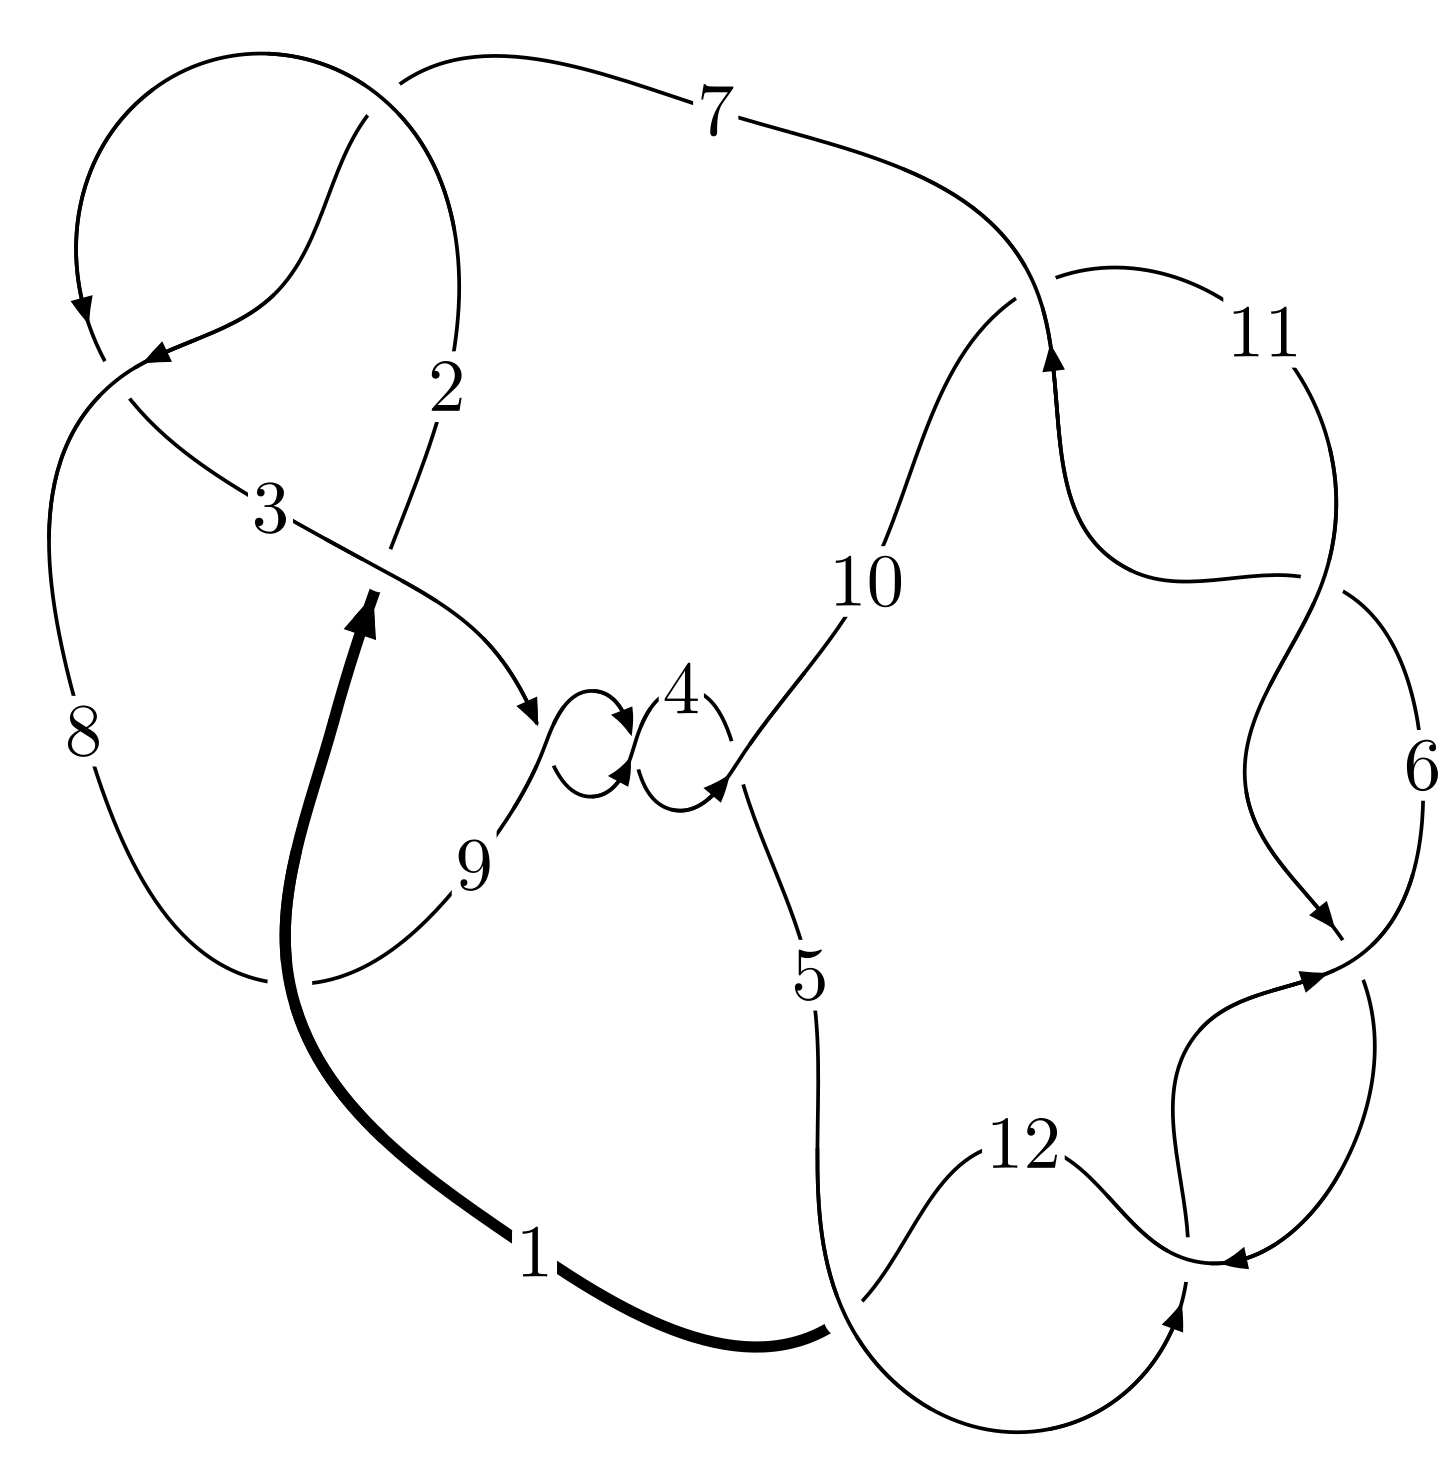
\includegraphics[width=112pt]{../../../GIT/diagram.site/Diagrams/png/1533_12a_0732.png}\\
\ \ \ A knot diagram\footnotemark}&
\allowdisplaybreaks
\textbf{Linearized knot diagam} \\
\cline{2-2}
 &
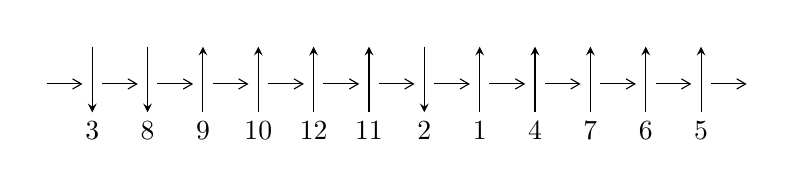
\begin{tikzpicture}[x=20pt, y=17pt]
	% nodes
	\node (C0) at (0, 0) {};
	\node (C1) at (1, 0) {};
	\node (C1U) at (1, +1) {};
	\node (C1D) at (1, -1) {3};

	\node (C2) at (2, 0) {};
	\node (C2U) at (2, +1) {};
	\node (C2D) at (2, -1) {8};

	\node (C3) at (3, 0) {};
	\node (C3U) at (3, +1) {};
	\node (C3D) at (3, -1) {9};

	\node (C4) at (4, 0) {};
	\node (C4U) at (4, +1) {};
	\node (C4D) at (4, -1) {10};

	\node (C5) at (5, 0) {};
	\node (C5U) at (5, +1) {};
	\node (C5D) at (5, -1) {12};

	\node (C6) at (6, 0) {};
	\node (C6U) at (6, +1) {};
	\node (C6D) at (6, -1) {11};

	\node (C7) at (7, 0) {};
	\node (C7U) at (7, +1) {};
	\node (C7D) at (7, -1) {2};

	\node (C8) at (8, 0) {};
	\node (C8U) at (8, +1) {};
	\node (C8D) at (8, -1) {1};

	\node (C9) at (9, 0) {};
	\node (C9U) at (9, +1) {};
	\node (C9D) at (9, -1) {4};

	\node (C10) at (10, 0) {};
	\node (C10U) at (10, +1) {};
	\node (C10D) at (10, -1) {7};

	\node (C11) at (11, 0) {};
	\node (C11U) at (11, +1) {};
	\node (C11D) at (11, -1) {6};

	\node (C12) at (12, 0) {};
	\node (C12U) at (12, +1) {};
	\node (C12D) at (12, -1) {5};
	\node (C13) at (13, 0) {};

	% arrows
	\draw[->,>={angle 60}]
	(C0) edge (C1) (C1) edge (C2) (C2) edge (C3) (C3) edge (C4) (C4) edge (C5) (C5) edge (C6) (C6) edge (C7) (C7) edge (C8) (C8) edge (C9) (C9) edge (C10) (C10) edge (C11) (C11) edge (C12) (C12) edge (C13) ;	\draw[->,>=stealth]
	(C1U) edge (C1D) (C2U) edge (C2D) (C3D) edge (C3U) (C4D) edge (C4U) (C5D) edge (C5U) (C6D) edge (C6U) (C7U) edge (C7D) (C8D) edge (C8U) (C9D) edge (C9U) (C10D) edge (C10U) (C11D) edge (C11U) (C12D) edge (C12U) ;
	\end{tikzpicture} \\
\hhline{~~} \\& 
\textbf{Solving Sequence} \\ \cline{2-2} 
 &
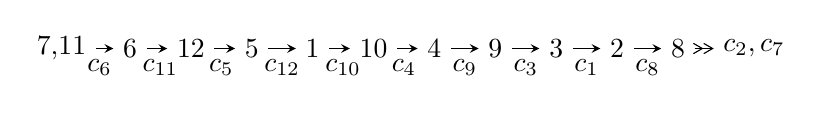
\begin{tikzpicture}[x=22pt, y=7pt]
	% node
	\node (A0) at (-1/8, 0) {7,11};
	\node (A1) at (1, 0) {6};
	\node (A2) at (2, 0) {12};
	\node (A3) at (3, 0) {5};
	\node (A4) at (4, 0) {1};
	\node (A5) at (5, 0) {10};
	\node (A6) at (6, 0) {4};
	\node (A7) at (7, 0) {9};
	\node (A8) at (8, 0) {3};
	\node (A9) at (9, 0) {2};
	\node (A10) at (10, 0) {8};
	\node (C1) at (1/2, -1) {$c_{6}$};
	\node (C2) at (3/2, -1) {$c_{11}$};
	\node (C3) at (5/2, -1) {$c_{5}$};
	\node (C4) at (7/2, -1) {$c_{12}$};
	\node (C5) at (9/2, -1) {$c_{10}$};
	\node (C6) at (11/2, -1) {$c_{4}$};
	\node (C7) at (13/2, -1) {$c_{9}$};
	\node (C8) at (15/2, -1) {$c_{3}$};
	\node (C9) at (17/2, -1) {$c_{1}$};
	\node (C10) at (19/2, -1) {$c_{8}$};
	\node (A11) at (45/4, 0) {$c_{2},c_{7}$};

	% edge
	\draw[->,>=stealth]	
	(A0) edge (A1) (A1) edge (A2) (A2) edge (A3) (A3) edge (A4) (A4) edge (A5) (A5) edge (A6) (A6) edge (A7) (A7) edge (A8) (A8) edge (A9) (A9) edge (A10) ;
	\draw[->>,>={angle 60}]	
	(A10) edge (A11);
\end{tikzpicture} \\ 

\end{tabular} \\

\footnotetext{
The image of knot diagram is generated by the software ``\textbf{Draw programme}" developed by Andrew Bartholomew(\url{http://www.layer8.co.uk/maths/draw/index.htm\#Running-draw}), where we modified some parts for our purpose(\url{https://github.com/CATsTAILs/LinksPainter}).
}\phantom \\ \newline 
\centering \textbf{Ideals for irreducible components\footnotemark of $X_{\text{par}}$} 
 
\begin{align*}
I^u_{1}&=\langle 
u^{47}+u^{46}+\cdots+2 u+1\rangle \\
\\
\end{align*}
\raggedright * 1 irreducible components of $\dim_{\mathbb{C}}=0$, with total 47 representations.\\
\footnotetext{All coefficients of polynomials are rational numbers. But the coefficients are sometimes approximated in decimal forms when there is not enough margin.}
\newpage
\renewcommand{\arraystretch}{1}
\centering \section*{I. $I^u_{1}= \langle u^{47}+u^{46}+\cdots+2 u+1 \rangle$}
\flushleft \textbf{(i) Arc colorings}\\
\begin{tabular}{m{7pt} m{180pt} m{7pt} m{180pt} }
\flushright $a_{7}=$&$\begin{pmatrix}1\\0\end{pmatrix}$ \\
\flushright $a_{11}=$&$\begin{pmatrix}0\\u\end{pmatrix}$ \\
\flushright $a_{6}=$&$\begin{pmatrix}1\\u^2\end{pmatrix}$ \\
\flushright $a_{12}=$&$\begin{pmatrix}u\\u^3+u\end{pmatrix}$ \\
\flushright $a_{5}=$&$\begin{pmatrix}u^2+1\\u^4+2 u^2\end{pmatrix}$ \\
\flushright $a_{1}=$&$\begin{pmatrix}u^3+2 u\\u^5+3 u^3+u\end{pmatrix}$ \\
\flushright $a_{10}=$&$\begin{pmatrix}- u\\u\end{pmatrix}$ \\
\flushright $a_{4}=$&$\begin{pmatrix}- u^6-3 u^4+1\\u^6+4 u^4+3 u^2\end{pmatrix}$ \\
\flushright $a_{9}=$&$\begin{pmatrix}u^{11}+6 u^9+10 u^7+2 u^5-3 u^3-2 u\\- u^{11}-7 u^9-16 u^7-13 u^5-3 u^3+u\end{pmatrix}$ \\
\flushright $a_{3}=$&$\begin{pmatrix}u^{16}+9 u^{14}+29 u^{12}+38 u^{10}+13 u^8-10 u^6-12 u^4-2 u^2+1\\- u^{16}-10 u^{14}-38 u^{12}-68 u^{10}-58 u^8-20 u^6+4 u^4+4 u^2\end{pmatrix}$ \\
\flushright $a_{2}=$&$\begin{pmatrix}- u^{37}-22 u^{35}+\cdots+10 u^3+u\\u^{37}+23 u^{35}+\cdots- u^3+u\end{pmatrix}$ \\
\flushright $a_{8}=$&$\begin{pmatrix}u^{19}+12 u^{17}+\cdots-11 u^3-2 u\\u^{21}+13 u^{19}+\cdots-7 u^3+u\end{pmatrix}$\\&\end{tabular}
\flushleft \textbf{(ii) Obstruction class $= -1$}\\~\\
\flushleft \textbf{(iii) Cusp Shapes $= 4 u^{46}+4 u^{45}+\cdots-4 u+10$}\\~\\
\newpage\renewcommand{\arraystretch}{1}
\flushleft \textbf{(iv) u-Polynomials at the component}\newline \\
\begin{tabular}{m{50pt}|m{274pt}}
Crossings & \hspace{64pt}u-Polynomials at each crossing \\
\hline $$\begin{aligned}c_{1}\end{aligned}$$&$\begin{aligned}
&u^{47}+21 u^{46}+\cdots+4 u+1
\end{aligned}$\\
\hline $$\begin{aligned}c_{2},c_{7}\end{aligned}$$&$\begin{aligned}
&u^{47}+u^{46}+\cdots+2 u^2-1
\end{aligned}$\\
\hline $$\begin{aligned}c_{3},c_{4},c_{9}\end{aligned}$$&$\begin{aligned}
&u^{47}- u^{46}+\cdots+19 u^2-4
\end{aligned}$\\
\hline $$\begin{aligned}c_{5},c_{6},c_{10}\\c_{11},c_{12}\end{aligned}$$&$\begin{aligned}
&u^{47}- u^{46}+\cdots+2 u-1
\end{aligned}$\\
\hline $$\begin{aligned}c_{8}\end{aligned}$$&$\begin{aligned}
&u^{47}+3 u^{46}+\cdots+4 u+1
\end{aligned}$\\
\hline
\end{tabular}\\~\\
\newpage\renewcommand{\arraystretch}{1}
\flushleft \textbf{(v) Riley Polynomials at the component}\newline \\
\begin{tabular}{m{50pt}|m{274pt}}
Crossings & \hspace{64pt}Riley Polynomials at each crossing \\
\hline $$\begin{aligned}c_{1}\end{aligned}$$&$\begin{aligned}
&y^{47}+11 y^{46}+\cdots-24 y-1
\end{aligned}$\\
\hline $$\begin{aligned}c_{2},c_{7}\end{aligned}$$&$\begin{aligned}
&y^{47}-21 y^{46}+\cdots+4 y-1
\end{aligned}$\\
\hline $$\begin{aligned}c_{3},c_{4},c_{9}\end{aligned}$$&$\begin{aligned}
&y^{47}-45 y^{46}+\cdots+152 y-16
\end{aligned}$\\
\hline $$\begin{aligned}c_{5},c_{6},c_{10}\\c_{11},c_{12}\end{aligned}$$&$\begin{aligned}
&y^{47}+59 y^{46}+\cdots+4 y-1
\end{aligned}$\\
\hline $$\begin{aligned}c_{8}\end{aligned}$$&$\begin{aligned}
&y^{47}- y^{46}+\cdots+48 y-1
\end{aligned}$\\
\hline
\end{tabular}\\~\\
\newpage\flushleft \textbf{(vi) Complex Volumes and Cusp Shapes}
$$\begin{array}{c|c|c}  
\text{Solutions to }I^u_{1}& \I (\text{vol} + \sqrt{-1}CS) & \text{Cusp shape}\\
 \hline 
\begin{aligned}
u &= -0.413784 + 0.877713 I\end{aligned}
 & \phantom{-}2.77094 - 10.32890 I & \phantom{-}4.55615 + 8.72539 I \\ \hline\begin{aligned}
u &= -0.413784 - 0.877713 I\end{aligned}
 & \phantom{-}2.77094 + 10.32890 I & \phantom{-}4.55615 - 8.72539 I \\ \hline\begin{aligned}
u &= \phantom{-}0.195276 + 0.942019 I\end{aligned}
 & -4.26421 + 6.13092 I & -0.95567 - 8.26497 I \\ \hline\begin{aligned}
u &= \phantom{-}0.195276 - 0.942019 I\end{aligned}
 & -4.26421 - 6.13092 I & -0.95567 + 8.26497 I \\ \hline\begin{aligned}
u &= \phantom{-}0.413997 + 0.861943 I\end{aligned}
 & \phantom{-}4.64721 + 5.04866 I & \phantom{-}7.42319 - 4.27573 I \\ \hline\begin{aligned}
u &= \phantom{-}0.413997 - 0.861943 I\end{aligned}
 & \phantom{-}4.64721 - 5.04866 I & \phantom{-}7.42319 + 4.27573 I \\ \hline\begin{aligned}
u &= \phantom{-}0.088069 + 0.951448 I\end{aligned}
 & -5.29996 - 0.71896 I & -4.01239 + 0.13887 I \\ \hline\begin{aligned}
u &= \phantom{-}0.088069 - 0.951448 I\end{aligned}
 & -5.29996 + 0.71896 I & -4.01239 - 0.13887 I \\ \hline\begin{aligned}
u &= -0.371801 + 0.847703 I\end{aligned}
 & -0.66504 - 3.24376 I & \phantom{-}1.24977 + 4.19607 I \\ \hline\begin{aligned}
u &= -0.371801 - 0.847703 I\end{aligned}
 & -0.66504 + 3.24376 I & \phantom{-}1.24977 - 4.19607 I \\ \hline\begin{aligned}
u &= \phantom{-}0.418667 + 0.819399 I\end{aligned}
 & \phantom{-}4.90772 + 2.01411 I & \phantom{-}7.94310 - 3.89227 I \\ \hline\begin{aligned}
u &= \phantom{-}0.418667 - 0.819399 I\end{aligned}
 & \phantom{-}4.90772 - 2.01411 I & \phantom{-}7.94310 + 3.89227 I \\ \hline\begin{aligned}
u &= -0.422632 + 0.799038 I\end{aligned}
 & \phantom{-}3.24960 + 3.24336 I & \phantom{-}5.51628 - 0.96386 I \\ \hline\begin{aligned}
u &= -0.422632 - 0.799038 I\end{aligned}
 & \phantom{-}3.24960 - 3.24336 I & \phantom{-}5.51628 + 0.96386 I \\ \hline\begin{aligned}
u &= -0.166444 + 0.877591 I\end{aligned}
 & -2.03526 - 1.97557 I & \phantom{-}2.70543 + 4.55475 I \\ \hline\begin{aligned}
u &= -0.166444 - 0.877591 I\end{aligned}
 & -2.03526 + 1.97557 I & \phantom{-}2.70543 - 4.55475 I \\ \hline\begin{aligned}
u &= -0.173002 + 0.658242 I\end{aligned}
 & -0.78945 - 1.82375 I & \phantom{-}5.03537 + 5.41712 I \\ \hline\begin{aligned}
u &= -0.173002 - 0.658242 I\end{aligned}
 & -0.78945 + 1.82375 I & \phantom{-}5.03537 - 5.41712 I \\ \hline\begin{aligned}
u &= -0.632705 + 0.037024 I\end{aligned}
 & \phantom{-}5.54952 - 6.80116 I & \phantom{-}9.39680 + 5.30944 I \\ \hline\begin{aligned}
u &= -0.632705 - 0.037024 I\end{aligned}
 & \phantom{-}5.54952 + 6.80116 I & \phantom{-}9.39680 - 5.30944 I \\ \hline\begin{aligned}
u &= \phantom{-}0.631119 + 0.020188 I\end{aligned}
 & \phantom{-}7.32256 + 1.52528 I & \phantom{-}12.11554 - 0.46181 I \\ \hline\begin{aligned}
u &= \phantom{-}0.631119 - 0.020188 I\end{aligned}
 & \phantom{-}7.32256 - 1.52528 I & \phantom{-}12.11554 + 0.46181 I \\ \hline\begin{aligned}
u &= -0.585855\phantom{ +0.000000I}\end{aligned}
 & \phantom{-}1.90017\phantom{ +0.000000I} & \phantom{-}6.44170\phantom{ +0.000000I} \\ \hline\begin{aligned}
u &= \phantom{-}0.263626 + 0.379028 I\end{aligned}
 & -1.33756 - 1.71540 I & \phantom{-}3.14465 - 0.50606 I \\ \hline\begin{aligned}
u &= \phantom{-}0.263626 - 0.379028 I\end{aligned}
 & -1.33756 + 1.71540 I & \phantom{-}3.14465 + 0.50606 I \\ \hline\begin{aligned}
u &= \phantom{-}0.408286 + 0.210597 I\end{aligned}
 & -0.73079 + 4.11365 I & \phantom{-}6.43864 - 8.58454 I \\ \hline\begin{aligned}
u &= \phantom{-}0.408286 - 0.210597 I\end{aligned}
 & -0.73079 - 4.11365 I & \phantom{-}6.43864 + 8.58454 I \\ \hline\begin{aligned}
u &= -0.368463 + 0.084232 I\end{aligned}
 & \phantom{-}0.852973 - 0.196059 I & \phantom{-}12.38641 + 2.18387 I \\ \hline\begin{aligned}
u &= -0.368463 - 0.084232 I\end{aligned}
 & \phantom{-}0.852973 + 0.196059 I & \phantom{-}12.38641 - 2.18387 I \\ \hline\begin{aligned}
u &= -0.01412 + 1.64039 I\end{aligned}
 & -8.92297 - 2.26281 I & \phantom{-0.000000 } 0\\
 \hline 
 \end{array}$$\newpage$$\begin{array}{c|c|c}  
\text{Solutions to }I^u_{1}& \I (\text{vol} + \sqrt{-1}CS) & \text{Cusp shape}\\
 \hline 
\begin{aligned}
u &= -0.01412 - 1.64039 I\end{aligned}
 & -8.92297 + 2.26281 I & \phantom{-0.000000 } 0 \\ \hline\begin{aligned}
u &= -0.10060 + 1.64581 I\end{aligned}
 & -5.17503 + 1.32295 I & \phantom{-0.000000 } 0 \\ \hline\begin{aligned}
u &= -0.10060 - 1.64581 I\end{aligned}
 & -5.17503 - 1.32295 I & \phantom{-0.000000 } 0 \\ \hline\begin{aligned}
u &= \phantom{-}0.10339 + 1.65410 I\end{aligned}
 & -3.64160 + 3.95604 I & \phantom{-0.000000 } 0 \\ \hline\begin{aligned}
u &= \phantom{-}0.10339 - 1.65410 I\end{aligned}
 & -3.64160 - 3.95604 I & \phantom{-0.000000 } 0 \\ \hline\begin{aligned}
u &= -0.09363 + 1.67036 I\end{aligned}
 & -9.45217 - 4.99818 I & \phantom{-0.000000 } 0 \\ \hline\begin{aligned}
u &= -0.09363 - 1.67036 I\end{aligned}
 & -9.45217 + 4.99818 I & \phantom{-0.000000 } 0 \\ \hline\begin{aligned}
u &= \phantom{-}0.10750 + 1.66999 I\end{aligned}
 & -4.14651 + 7.03674 I & \phantom{-0.000000 } 0 \\ \hline\begin{aligned}
u &= \phantom{-}0.10750 - 1.66999 I\end{aligned}
 & -4.14651 - 7.03674 I & \phantom{-0.000000 } 0 \\ \hline\begin{aligned}
u &= -0.10893 + 1.67541 I\end{aligned}
 & -6.10861 - 12.33850 I & \phantom{-0.000000 } 0 \\ \hline\begin{aligned}
u &= -0.10893 - 1.67541 I\end{aligned}
 & -6.10861 + 12.33850 I & \phantom{-0.000000 } 0 \\ \hline\begin{aligned}
u &= -0.03693 + 1.68229 I\end{aligned}
 & -11.09350 - 2.72228 I & \phantom{-0.000000 } 0 \\ \hline\begin{aligned}
u &= -0.03693 - 1.68229 I\end{aligned}
 & -11.09350 + 2.72228 I & \phantom{-0.000000 } 0 \\ \hline\begin{aligned}
u &= \phantom{-}0.04483 + 1.69525 I\end{aligned}
 & -13.5927 + 7.0408 I & \phantom{-0.000000 } 0 \\ \hline\begin{aligned}
u &= \phantom{-}0.04483 - 1.69525 I\end{aligned}
 & -13.5927 - 7.0408 I & \phantom{-0.000000 } 0 \\ \hline\begin{aligned}
u &= \phantom{-}0.02120 + 1.69620 I\end{aligned}
 & -14.6803 - 0.2975 I & \phantom{-0.000000 } 0 \\ \hline\begin{aligned}
u &= \phantom{-}0.02120 - 1.69620 I\end{aligned}
 & -14.6803 + 0.2975 I & \phantom{-0.000000 } 0\\
 \hline 
 \end{array}$$\newpage
\newpage\renewcommand{\arraystretch}{1}
\centering \section*{ II. u-Polynomials}
\begin{tabular}{m{50pt}|m{274pt}}
Crossings & \hspace{64pt}u-Polynomials at each crossing \\
\hline $$\begin{aligned}c_{1}\end{aligned}$$&$\begin{aligned}
&u^{47}+21 u^{46}+\cdots+4 u+1
\end{aligned}$\\
\hline $$\begin{aligned}c_{2},c_{7}\end{aligned}$$&$\begin{aligned}
&u^{47}+u^{46}+\cdots+2 u^2-1
\end{aligned}$\\
\hline $$\begin{aligned}c_{3},c_{4},c_{9}\end{aligned}$$&$\begin{aligned}
&u^{47}- u^{46}+\cdots+19 u^2-4
\end{aligned}$\\
\hline $$\begin{aligned}c_{5},c_{6},c_{10}\\c_{11},c_{12}\end{aligned}$$&$\begin{aligned}
&u^{47}- u^{46}+\cdots+2 u-1
\end{aligned}$\\
\hline $$\begin{aligned}c_{8}\end{aligned}$$&$\begin{aligned}
&u^{47}+3 u^{46}+\cdots+4 u+1
\end{aligned}$\\
\hline
\end{tabular}\newpage\renewcommand{\arraystretch}{1}
\centering \section*{ III. Riley Polynomials}
\begin{tabular}{m{50pt}|m{274pt}}
Crossings & \hspace{64pt}Riley Polynomials at each crossing \\
\hline $$\begin{aligned}c_{1}\end{aligned}$$&$\begin{aligned}
&y^{47}+11 y^{46}+\cdots-24 y-1
\end{aligned}$\\
\hline $$\begin{aligned}c_{2},c_{7}\end{aligned}$$&$\begin{aligned}
&y^{47}-21 y^{46}+\cdots+4 y-1
\end{aligned}$\\
\hline $$\begin{aligned}c_{3},c_{4},c_{9}\end{aligned}$$&$\begin{aligned}
&y^{47}-45 y^{46}+\cdots+152 y-16
\end{aligned}$\\
\hline $$\begin{aligned}c_{5},c_{6},c_{10}\\c_{11},c_{12}\end{aligned}$$&$\begin{aligned}
&y^{47}+59 y^{46}+\cdots+4 y-1
\end{aligned}$\\
\hline $$\begin{aligned}c_{8}\end{aligned}$$&$\begin{aligned}
&y^{47}- y^{46}+\cdots+48 y-1
\end{aligned}$\\
\hline
\end{tabular}
\vskip 2pc
\end{document}